%% The following is a directive for TeXShop to indicate the main file
%%!TEX root = diss.tex
 
\chapter{Challenges}
\label{ch:Challenges}

\section{Methodology}
In this study, we aim to characterize the development challenges of IoT developers in a systematic way. More precisely, we want to answer the following research questions:
\begin{itemize}
\item {\verb|RQ1|}: What are the types of development challenges IoT developers face?
\item {\verb|RQ2|}: How frequent each of these development challenge are based on IoT developers' opinions?
\item {\verb|RQ3|}: What development challenges require more attention from the research community and the industry?
\end{itemize}

To answer these RQs, we devised the bug discussion analysis, IoT developer interviews and survey that we discussed in~\autoref{ch:bugs} to characterize the development challenges in the context of IoT. 

\subsection{GitHub Issues Discussions}
During the categorization of IoT bugs, we also read the entire GitHub discussion for each bug report and kept track of the challenges IoT developers are dealing with. We used the same tagging technique discussed in section {\autoref{interviewAnalysis} for analyzing challenges we observe while reading through GitHub discussions. Our goal was to come up with some examples and initial high-level categories of IoT development challenges . We aimed to use these initial data to lead the semi-structured interviews with IoT developers which will be discussed in the next section.


\subsection{Interviews}
During the interviews discussed in section \autoref{interviews4Bug}, we included open-ended questions about the challenges of IoT development as well. Although we had already tagged some possible challenges while reading through GitHub discussions during bug labeling, we employed these interviews to add new aspects of IoT development challenges to our data. Our semi-structured interviews helped us avoid being restricted to only code-level challenges and capture developers' high-level problems too. We could collect a more comprehensive set of IoT development challenges with inputs from developers of different IoT backgrounds during interviews. The participants, protocol, and analysis of interviews for the challenges section of interviews, was mostly the same as for the bugs section. The only major difference was that as included more open-ended questions about IoT development challenges. 

By using the categories we extracted from interviews and the examples we collected during bug labelling, we already had enough data to form the initial categories of IoT development challenges utilizing the protocol discussed in section \autoref{interviewProtocol}. 

\subsection{Survey}
We employed the survey discussed in section \autoref{survey4bug}  to validate the categories of challenges we had with a larger number of IoT developers. We also could collect more insights and examples for each category of IoT development challenges, which helped us to characterize them more comprehensively. 


\section{Findings}
In this section, we provide our findings regarding the challenges faced by IoT developers.

\subsection{Testing and Debugging Challenges}
\textbf{Relying on access to the real device}
According to seven interviewees, several GitHub issues (DEVICE-OS/1871, MYCONTROLLER/485, TESLA-API/43), and 74\% of survey participants, IoT developers rely on access to devices to test and debug their IoT system, by tasks such as manual reset or device output monitoring (P\textsubscript{2,3,7}).

\begin{lstlisting} [language=Java, caption={Steps to test a variable lag bug in DEVICE-OS/1567}, label={lst:varLag}] 
// Develoeprs need to flash a real device in order to test the fix
1- Flash LTE device with this system firmware and tinker
//Manual digital write to the physical device
2- Make a function call particle call <device> digitalwrite D7,LOW 
//Manual investigation of the device output
3- It should return 1 if successful   
4- Wait 3 minutes 
//repeat the scenario again
5- Make a function call particle call <device> digitalwrite D7,LOW
6- It should return 1 if successful 
\end{lstlisting}



Three interviewees (P\textsubscript{2}, P\textsubscript{3}, P\textsubscript{7}) mentioned that in some scenarios, they need access to the physical hardware to reset the device or investigate the output of the device for debugging.

 For instance, as it is shown in~\autoref{lst:varLag}, to test a fix for a variable lag related in an IoT device, developers need to do manual digital writes to the IoT device after some time intervals, and also investigate the output. GitHub discussions show that IoT developers go through these steps manually.
 
 Another example in the same project is show in~\autoref{lst:USBSOS}, where the IoT developers have to apply physical changes to the device, like plugging or unplugging the battery, and also observe the physical state of the device in order to make sure that the fix completely fixes the bug. 
 
 \begin{lstlisting} [language=Java, caption={Steps to test a USBSerial SOS issue in DEVICE-OS/1707}, label={lst:USBSOS}] 
// Develoeprs need battery-powered devices in order to test the fix
1- Flash the example application to a battery powered device
//Developers need to manually change the physical state of the device
2- Disconnect and reconnect the USB cable
//Manual investigation of the physical state of the device
3- Observe the LED status, whether it will enter SOS mode
\end{lstlisting}

This challenge is also observable in other bug reports in GitHub (DEVICE-OS/1871, MYCONTROLLER/485, HOMIE-ESP8266/242). 
One example is a developer saying "\emph{I need to check on my car to see what is returned by the API}" in discussions for TESLA-API/43.
In some scenarios, devices are out of reach or in hard-to-access locations thus making remote debugging more essential. 
Four interviewees believed that practical simulation solutions are required for better IoT testing and debugging. As P\textsubscript{5}, a middleware developer stated "\emph{IoT device vendors do not provide a mock of their devices, and we have to do reverse engineering on the actual hardware devices rather than working with the simulated ones.}" Also as P\textsubscript{5,8,9} stated, current simulation solutions in IoT are not mature enough and they are only valid for limited scenarios, such as testing high-level controllers or small unit tests, rather than being suitable for all levels of testing such as system testing.
 For instance, P\textsubscript{8} states "\emph{Device simulation can only help in either testing high-level controllers or small unit tests rather than helping with testing all functionalities of your system in integration with a Google NEST device as an example.}"
 In general, as P\textsubscript{5,9} also mentioned, compared to developing software within other ecosystems such as web platforms, where you can simulate server and browser in your local environment, simulation in IoT is not mature yet.
Some relevant challenges mentioned in the survey are \emph{affording to have all types of IoT devices}, \emph{complex custom logic for effective IoT device mocking and simulation}, and \emph{setting up test environments with IoT devices}. 

\textbf{Fault localization}
According to eight interviewees, nine survey comments, and also half of the survey participants, fault localization is a barrier due to lack of transparency in the operations of IoT systems. As P\textsubscript{7} mentioned "\emph{there is no environment that logs everything.}" One contributing factor to this is the difficulty of tracing executions of numerous external components in IoT systems. P\textsubscript{3} mentioned using open-source solutions just to be able to log everything. 

Another factor that impacts fault localization is the existence of hidden failures. As an example, P\textsubscript{7} mentioned "\emph{It's hard to recognize on the app that the temperature the device is reporting now is for several minutes ago.}" Also P\textsubscript{5} states "\emph{Usually, the bug is inconsequential until it is perceived at the end of the chain in the user interface.}"

Moreover, P\textsubscript{2,4} mentioned examples of failures that only show up after the device has worked for a specific amount of time (five minutes for P\textsubscript{2}, several hours for P\textsubscript{4}), which is also observed in GitHub issues (DEVICE-OS/1926, ZWAVE2MQTT/141, VSCP/207). This issue makes IoT failures more unpredictable and may hide developers' faults. Another issue toward fault localization is the lack of tools and developers' support. For instance, P\textsubscript{3} inspects device messages in bit-level by monitoring communications using Wireshark. P\textsubscript{2}, as a hardware platform developer, said "\emph{Since there is no feedback of errors or corruptions from devices, we've added some LEDs to them to track if something is working in the device level or not.}"  

According to the survey results, more than half of the IoT developers agree with the lack of transparency as a challenge for debugging IoT, and nine IoT developers mentioned fault localization as one of the main IoT developers' challenges in the survey comments.


\textbf{Reproducing IoT bugs}
In addition to observing several GitHub discussions (DITTO/414, TESLA-API/68), we collected four tags from interviews, and three survey comments regarding the challenge of reproducing IoT bugs. Besides the already mentioned factors which harden bug reproduction, such as limited access to devices or hidden failures, some bugs only happen with a specific device setting or with certain environments of the IoT system. IoT developers cannot reproduce these bugs unless they have exactly the same setting or environment. For instance, a survey comment indicated "\emph{It's hard to reproduce some memory-related bugs in X86 devices when they have ASLR enabled.}"
% due to existence of ASLR mechanism in these devices that interfere with these bugs
Also, we observed other examples such as TEMPERATURE-MACHINE/13: "\emph{I can reproduce the bug with the help of ice packs taken at three different temperatures from my freezer.}"

\textbf{Combinatorial explosion}
In addition to all the evolving components in traditional software, such as libraries and operating systems, there are more changing factors in IoT systems. Hardware devices produced by various manufacturers with different standards, device integration middlewares, and communication protocols are some examples of these extra changing factors in IoT. With all these components releasing new versions at a specific rate, a combinatorial explosion problem is likely to happen when developers want to cover all possible combinations with test cases.
One relevant statement is "\emph{I do not have all kinds of bulbs, remotes, and sensors, so I could be completely wrong!}" in a GitHub discussion (PYTRADFRI/135). We could collect eight tags come from four interviewees and two tags from survey comments regarding the challenge of combinatorial testing. As one example, P\textsubscript{9} said "\emph{We have to test with 10 or 15 different devices each time.}" Also, 80 percent of survey respondents agree with the combinatorial explosion as a testing challenge for IoT developers, and P\textsubscript{8} mentioned it as the most severe testing challenge. 

~\autoref{lst:usbBug} shows how presence of physical devices can increase the test search space. In addition to regular tests that all systems have, IoT developers have to spend some additional time on writing and executing tests that cover interaction scenarios with physical devices.

\begin{lstlisting} [language=Java, caption={All different scenarios developers have to check, just to test a fix provided for a USB messaging bug in DEVICE-OS/1871}, label={lst:usbBug}] 
 - State changes are sane when the device is powered with USB cable in.
 - State changes are sane when the device is powered with no USB cable in (powered through VIN).
 - State changes are sane when USB cable is unplugged.
 - State changes are sane when USB cable is plugged back.
 - State changes are sane when Serial.end() is called and cable is unplugged and re-plugged. 
 - State changes are sane once Serial.begin() is called after.
 - State changes are sane once Serial.end() is called, cable is unplugged, Serial.begin() is called, and cable is plugged back.
\end{lstlisting}

\textbf{Testing and debugging edge-cases}
Covering large-scale scenarios (e.g. too many devices) and exceptional cases (e.g. temperatures below zero) add to the test coverage obstacles. This challenge is mentioned by four interviewees, three survey participants, and observed in several GitHub discussions (DEVICE-OS/1926, TEMPERATURE-MACHINE/13). As one example, P\textsubscript{4} said "\emph{We should put effort to write proper tests against concurrency issues since we should be able to handle 140,000 HTTP requests per second because our IoT system is deployed in different cities.}" Additionally, this challenge is the most experienced testing challenge (83\% of respondents). 



 \begin{figure}%[h]
  \centering
   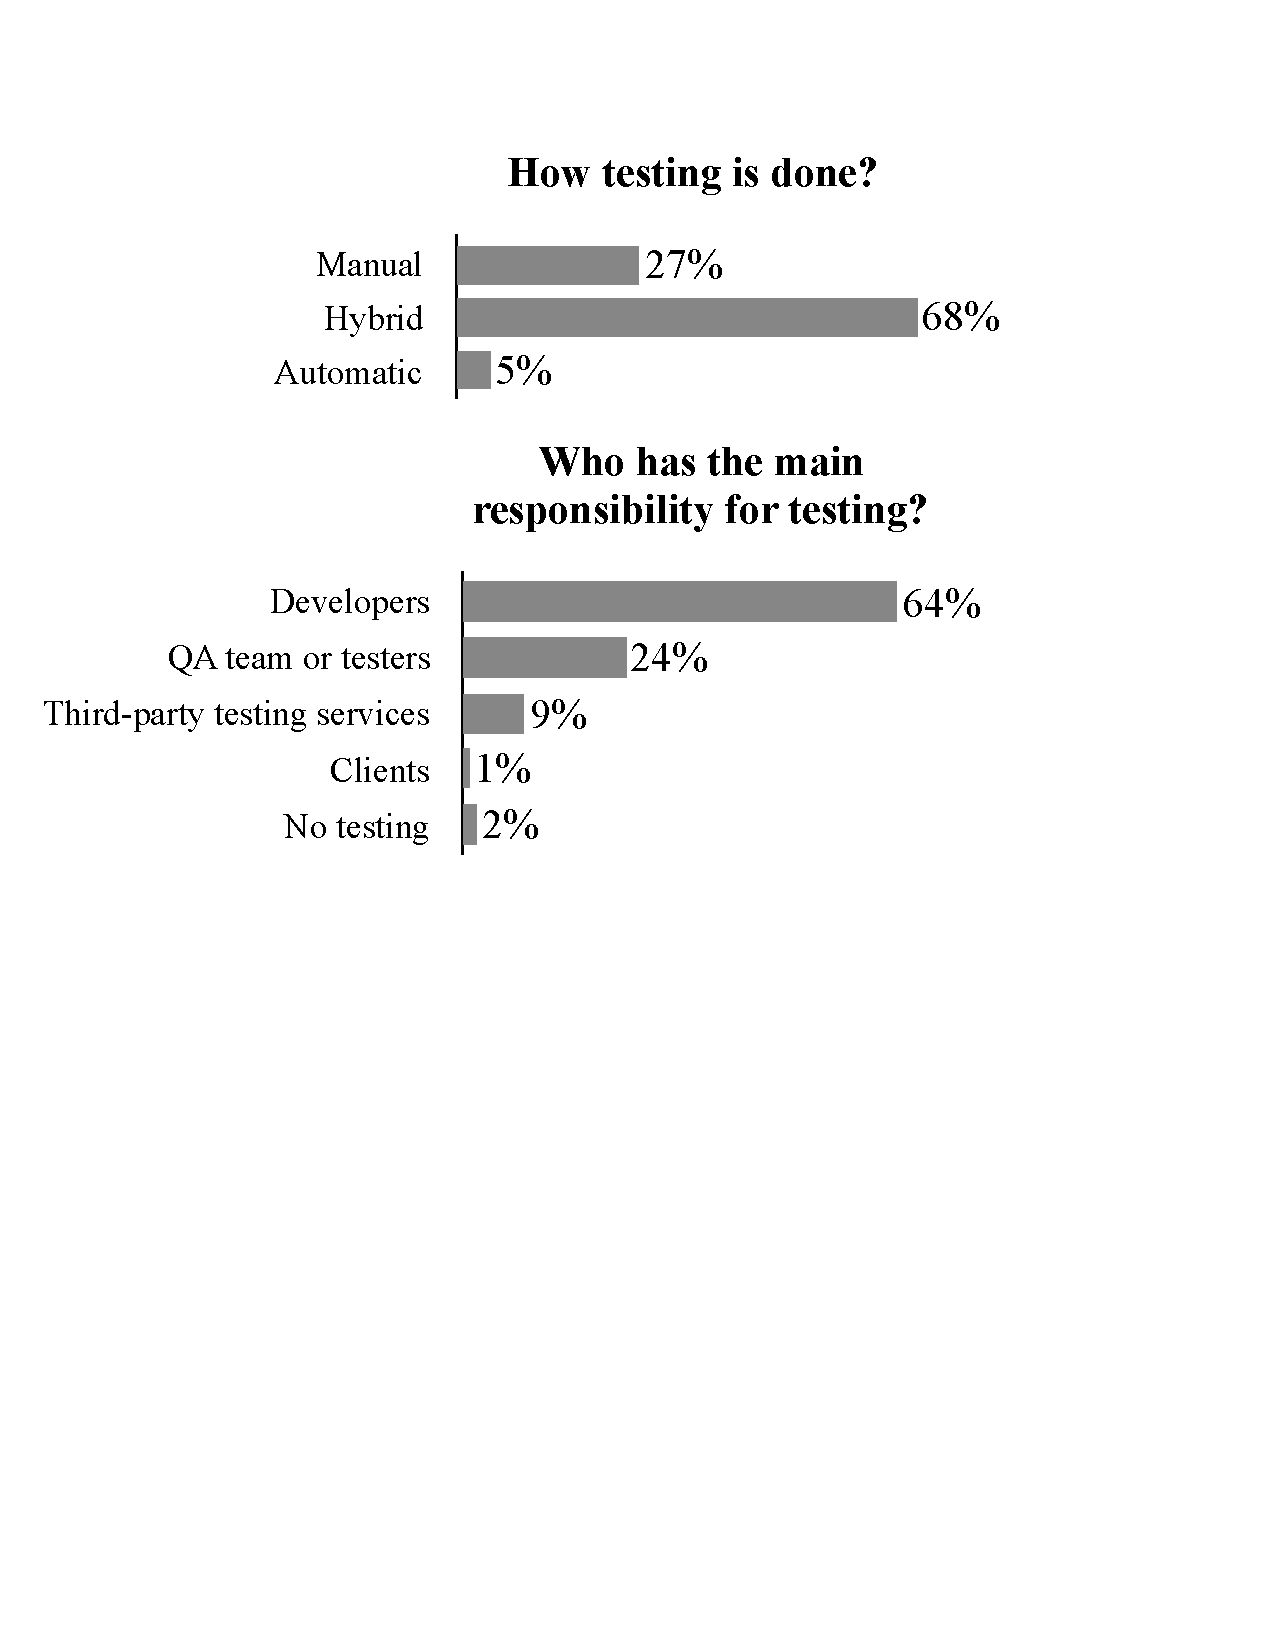
\includegraphics[width=\linewidth]{imgs/testing.pdf}
  \caption{Survey responses about how testing is done in IoT projects.
  }
  \label{fig:testing}
\end{figure}



\textbf{Immature testing culture}
Figure~\ref{fig:testing} shows an over-reliant on IoT developers for testing as 64\% of participants mentioned developers are the main testers in their IoT project. After developers, the main responsibility of testing is for QA teams (24\%), third-party testing services (9\%), and clients (1\%). Furthermore, two\% of participants have reported that they don'y have sophisticated testing.

Specially in the open-source community, developers rely on clients, who have a more diverse set of devices, for testing and debugging (ZWAVE2MQTT/141). We witnessed several examples of asking the users who reported the bug to test with a certain devices and report it back to the developers, since the developers don't have the actual devices. There are several quotes during interviews from open-source developers such as "\emph{The platform is well-tested from the software side and usually, the bugs are because of unknown hardware issues.}" or another open-source IoT developer that mentioned "\emph{We don't know what practices are good for hardware testing and lots of bugs are discovered by the community.}"

As P\textsubscript{6}, a developer of a popular IoT project with near 7K stars, stated "\emph{We do not have a QA team. it's up to developers to do testing, either manually or writing automated tests.}" Often, software developers do not have the skills to test the hardware side. P\textsubscript{9}, a software developer of an IoT platform with 1.5K stars, told that the bottle-neck of their IoT platform is testing the hardware side since they do not have sufficient knowledge for tools and practices of hardware testing.

As Figure~\ref{fig:testing} shows, IoT testing highly depends on manual tasks as only 5\% of participants reported testing completely automatic. Also, during interviews, four interviewees mentioned manual approaches for IoT testing. According to the survey respondents, the most adopted IoT testing approach is hybrid strategies. An example of such an approach is described by one IoT developer "\emph{Services which don't interact with devices directly are tested automatically, but checking the entire platform with devices requires manual testing.}" 

Based on our survey results, only 5\% IoT developers use complete automated testing. Around 27\% of IoT developers rely on complete manual testing while the rest (68\%) use a hybrid approach. 


 \begin{figure}%[h]
  \centering
   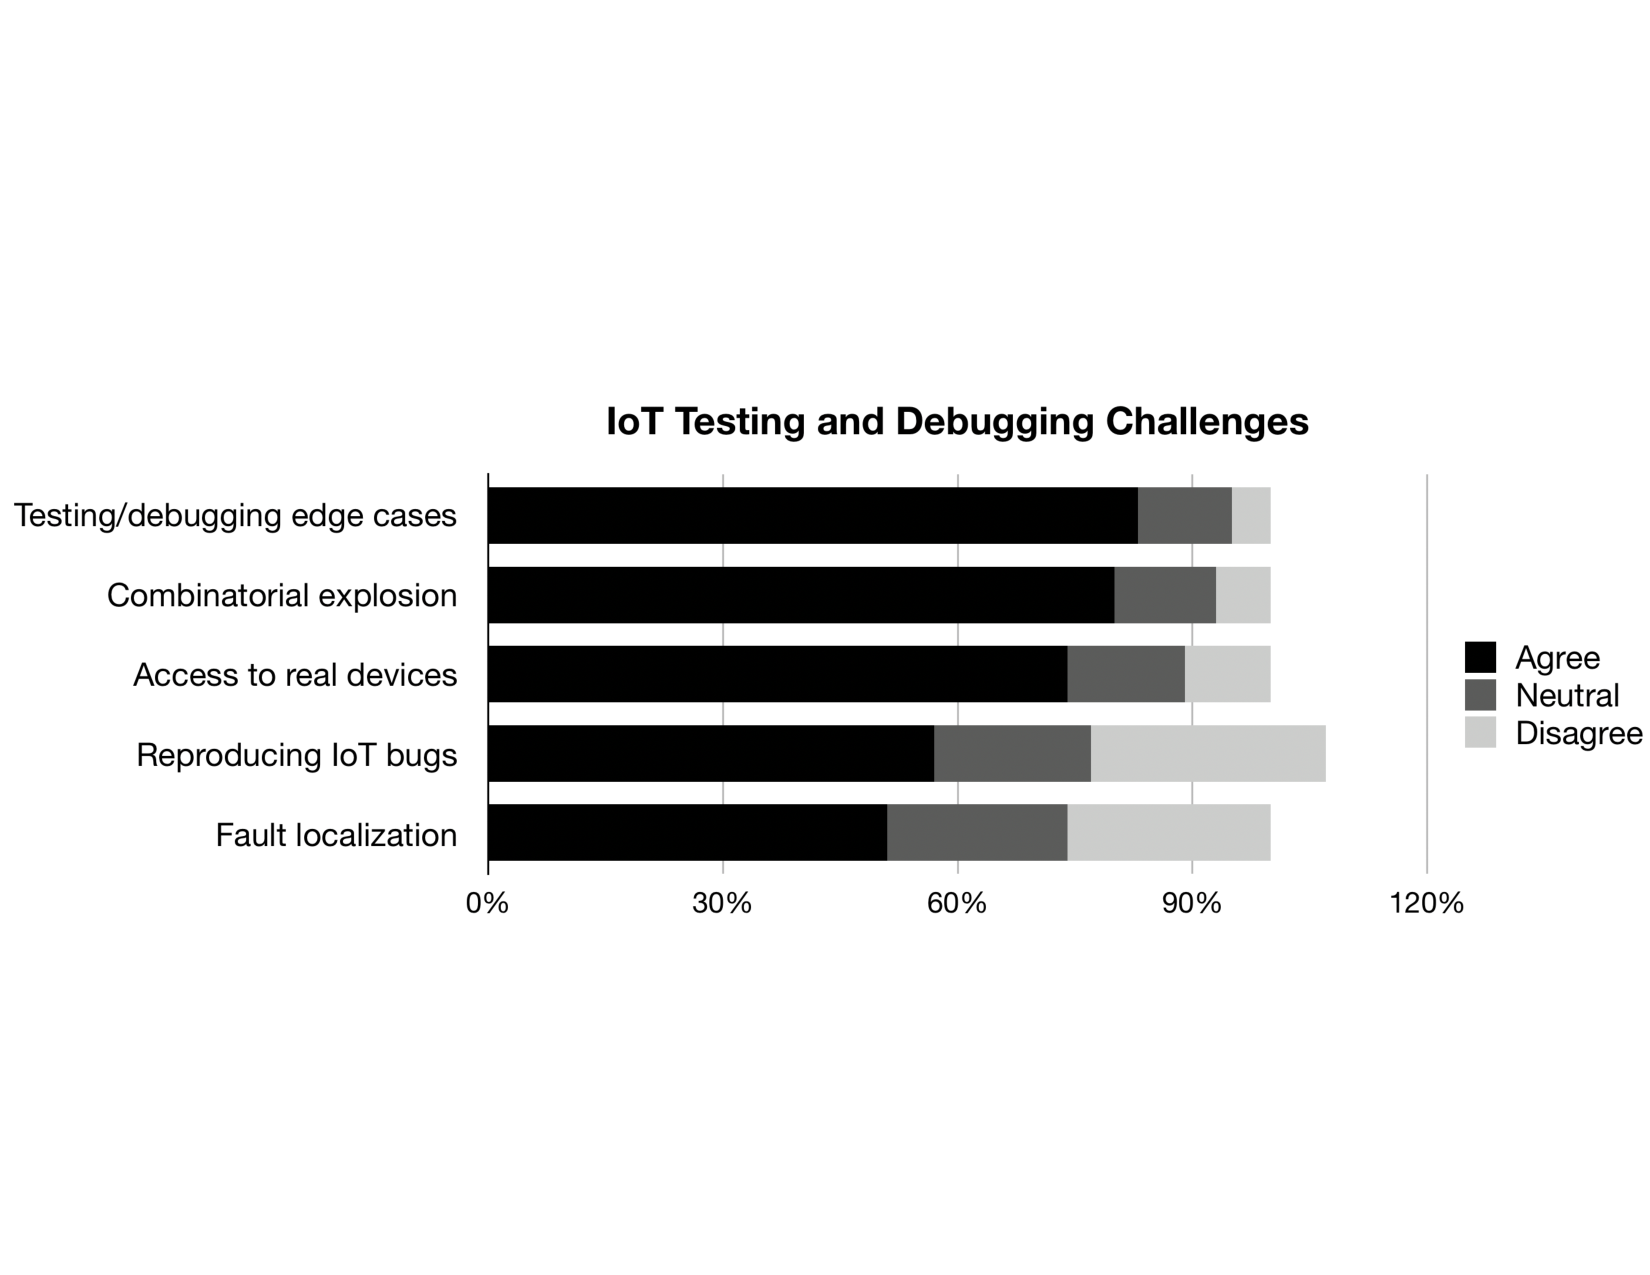
\includegraphics[width=\linewidth]{imgs/survey1}
  \caption{Survey responses about challenges of testing and debugging in IoT projects.}
  \label{fig:survey1}
\end{figure}


\subsection{Heterogeneity}
\textbf{Device and protocol fragmentation} Some of the IoT developers reported developing separately for each device or protocol in order to fulfill interoperability (P\textsubscript{2-5}, P\textsubscript{8}). For instance, P\textsubscript{3} stated he has to develop a distinct adapter for talking with each particular device. He mentioned \textit{"There is no guarantee that something that works with brand A also works with brand B."} On the other hand, P\textsubscript{6} noted that their platform is restricted to certain protocols instead of devices. Other developers mentioned fragmentation challenges by pointing out \emph{fragmentation on the same platform} and \emph{time to implement new technologies.} In addition, the majority of the interviewees (seven out of nine), 11 survey comments, and near half of the survey respondents find integration with a new IoT device or communication protocol challenging. 

The fragmentation issue can also be perceived by looking through GitHub issues. For instance, AZURE-IOT-SDK-C/815 happens due to minor timing differences between MQTT and AMQP protocols, and AZURE-IOT-SDK-C/213 is caused by different reliability of communication protocols as a developer says "\emph{I've never faced any issue with Ethernet connectivity, since its very stable, but WiFi and Cellular face so many issues.}"

\textbf{Third-party breaking changes}
Third-party changes challenge is mentioned by all interviewees (23 tags) and is agreed by 63\% of survey participants and also there are several comments in the survey about it (eight tags). Three interviewees stated that third-parties make breaking changes without prior notice. Also, P\textsubscript{5,8} mentioned examples where the third-party system stopped supporting a device or a service which caused breakage in their IoT system. Four interviewees (P\textsubscript{2,4,5,8}) explicitly mentioned that it's hard to keep pace with all the rapid changes from various third-parties such as device manufacturers. 

\textbf{Diversity of technologies, backgrounds, and requirements}
Challenges posed by the fundamental diversity of IoT technologies are the most repeated challenges among both interviews (30 tags) and survey comments (25 tags). Several participants mentioned that IoT development requires diverse development skills such as hardware programming and knowledge in dealing with network protocols.

Commonly, developers do not go through this learning curve: "\emph{developers tend to use protocols which they are familiar with but sometimes better solutions exist and developers do not know/use them.}" 

60\% of IoT developers agreed that it's challenging for them to learn and interpret different technologies and network protocols to be able to develop an IoT system.
One interesting theme emerged from interviews and the survey is making hardware and software developers with diverse backgrounds and skills work together (P\textsubscript{2-3,9}), and nine survey comments).
One challenge that is mentioned by participants is making embedded developers and cloud developers work independently with each other.
The consequences of inadequate backgrounds of developers are best described in another comment as it says "\emph{It causes a large number of devices to end up with security flaws, or the inability to deal with disconnections.}"

P\textsubscript{2,3,7,8} and several survey comments mentioned that it is hard to understand low-quality documentation of certain device manufacturers and interpret complex response payloads from particular devices. P\textsubscript{2,3} and two survey comments also mentioned that user requirements, as well as users' backgrounds and skills, can be very disparate and it's challenging to develop a generalized IoT system that can support all possible use cases. For instance, P\textsubscript{2} mentioned that they had to include more pins on their hardware and add support for obscured sensors to cover all user requirements. Other challenges are \emph{large search-space for selecting compatible devices or libraries} (P\textsubscript{5,7,8}), and \emph{dealing with diverse regulations and standards} (P\textsubscript{5,8}, and three survey comments).


 \begin{figure}%[h]
  \centering
   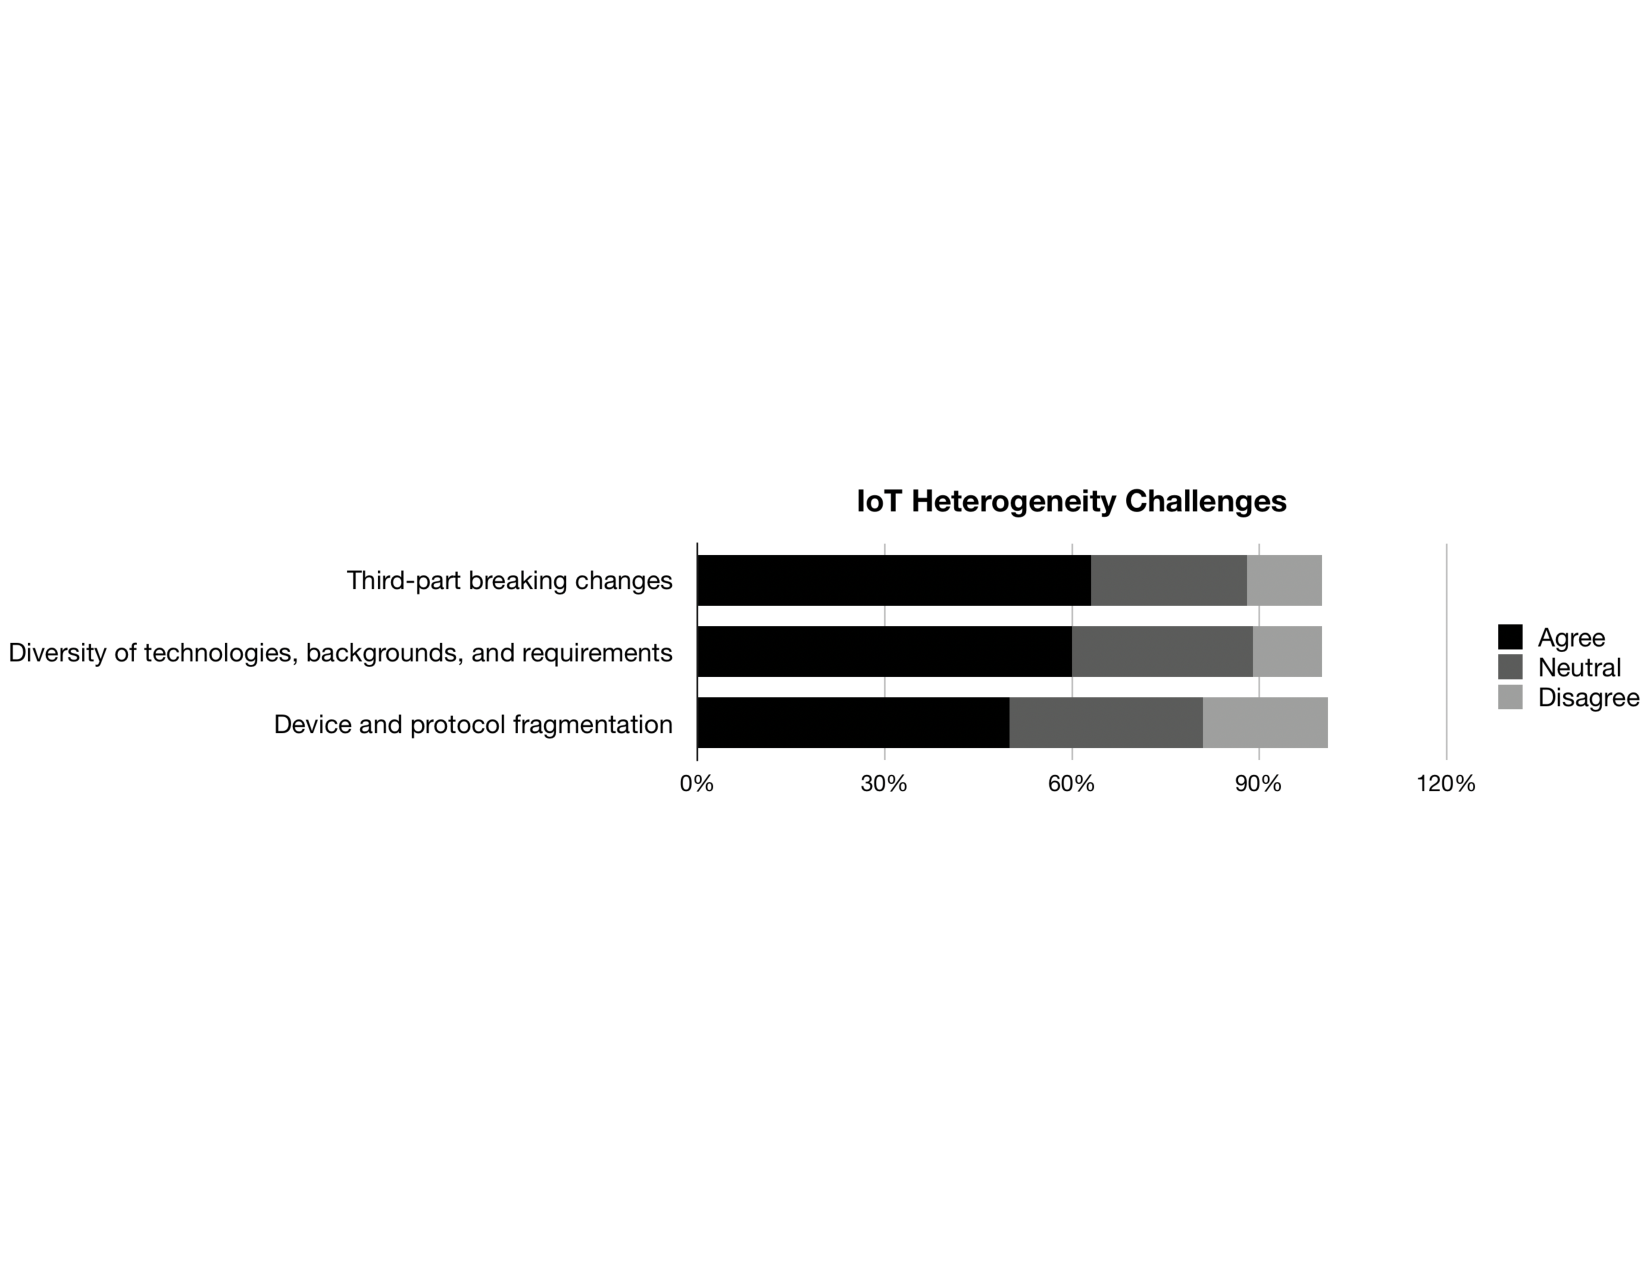
\includegraphics[width=\linewidth]{imgs/survey2}
  \caption{Survey responses about challenges related to hetereogenity in IoT projects.}
  \label{fig:survey2}
\end{figure}

\subsection{IoT security challenges}
Also, from a total of 14 participants who mentioned security-related challenges, six of them posed it as the most important challenge. Below we will describe the security challenges aspect of IoT development that we could gather from our survey.

\textbf{Complexity of IoT security}
First of all, 66\% of IoT developers find security a complicated task. Our interview participants mentioned security issues rooted in the device firmware (P\textsubscript{1,3,4}), network protocols (P\textsubscript{7,8}), and automation rules (P\textsubscript{6}).  Another emerged theme from our data is related to the challenge of end-to-end security, from the IoT device to the cloud. Other challenges mentioned are \emph{the complexity of the certification process}, \emph{supporting different use cases while following security protocols}, and \emph{existence of various attack surfaces}.

\textbf{Handling device-level security}
One of the main challenges, also mentioned by P\textsubscript{7}, is generating and storing access tokens within IoT devices that have processing and storage limitations. Similarly, near 60\% of IoT developers think that device constraints make security tasks challenging.  Some (P\textsubscript{8,9}) believe that the security of the local communication between the device and IoT gateway is usually underestimated while it can be highly insecure. As P\textsubscript{9} argued, "\emph{to make the development of the IoT system faster, developers don't consider the security of the local network.}"

\textbf{Handling security of external components}
As the survey results suggest, more than half of the IoT developers are not confident about the security of the third-party components, such as operating systems and libraries, used in their IoT system. 

 \begin{figure}%[h]
  \centering
   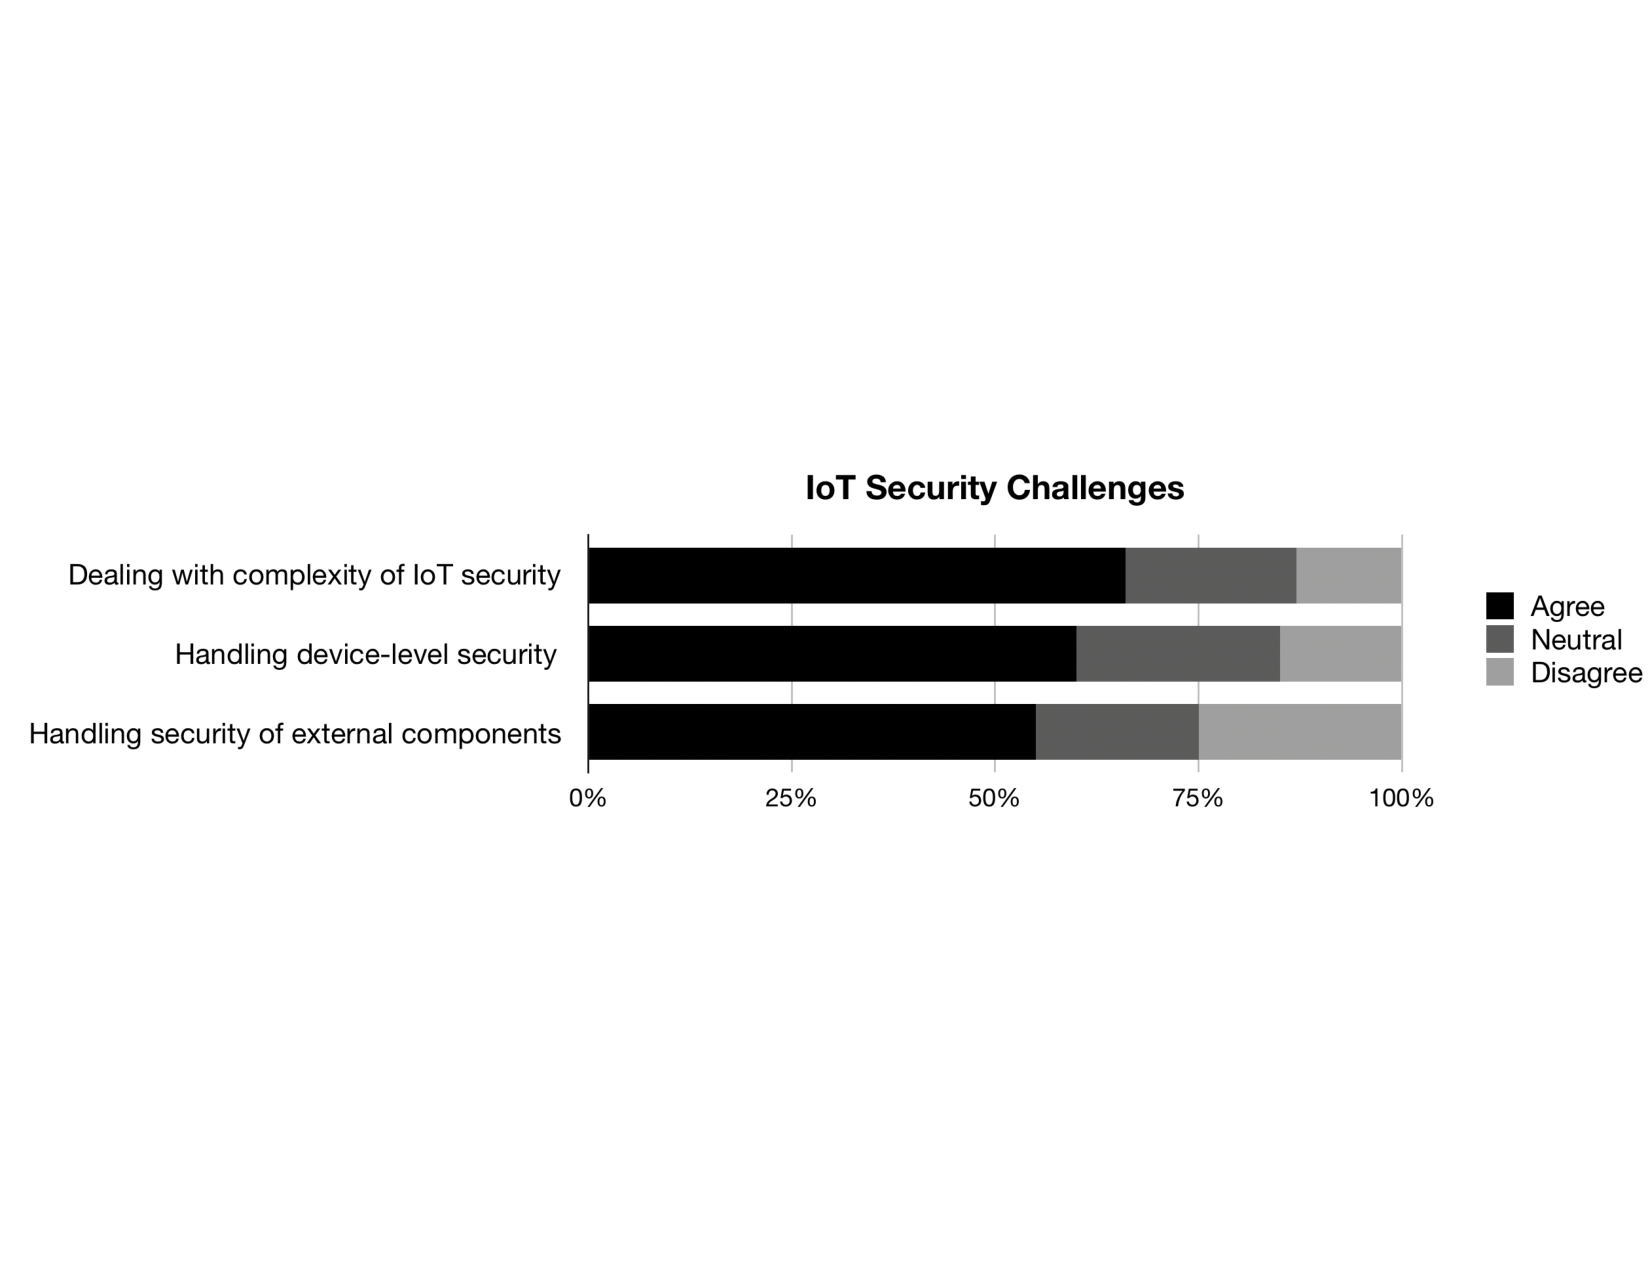
\includegraphics[width=\linewidth]{imgs/survey3}
  \caption{Survey responses about IoT security challenges.}
  \label{fig:survey3}
\end{figure}


\subsection{Other challenges}
\textbf{Releasing updates for IoT devices}  Half of the interviewees believe that releasing software upgrades or security patches for already shipped devices (P\textsubscript{5,8}) is inevitably challenging. Six IoT developers in the survey made comments such as \emph{getting critical updates installed on already sold devices}" or \emph{firmware updates in large deployments} regarding update challenges.

\textbf{Programming for constrained devices}
63\% of the participants agreed that device constraints make IoT development harder. Most IoT developers struggle to design and implement software in a way to consume less processing power and energy. Device limitations in different layers have also been mentioned by our interviewees (P\textsubscript{2,3,6,8}). 

The listing~\autoref{lst:USBSOS}, which is already discussed in testing challenges, is also pointing out the obstacles caused by device constraints. This bug is an example of how IoT developers should be ready for different physical states of the devices' battery (plugged, unplugged), and consider all scenarios when writing code. 

\textbf{Handling failures} An interesting theme that 62\% of our participants agreed with is the challenge of handling failures in IoT systems, in a way to avoid losing data and making the system unavailable. As P\textsubscript{4,5} and five IoT developers from the survey described, developers have to design the system to be tolerable to failures and data losses. \emph{Handling a backlog of sensor data in gateways or constraint devices in case of disconnections} (P\textsubscript{6}, ZWAVE2MQTT/141), and \emph{reducing mean-time-to-repair (MTTR) on already shipped devices} are some of the mentioned reliability challenges. 

 \begin{figure}%[h]
  \centering
   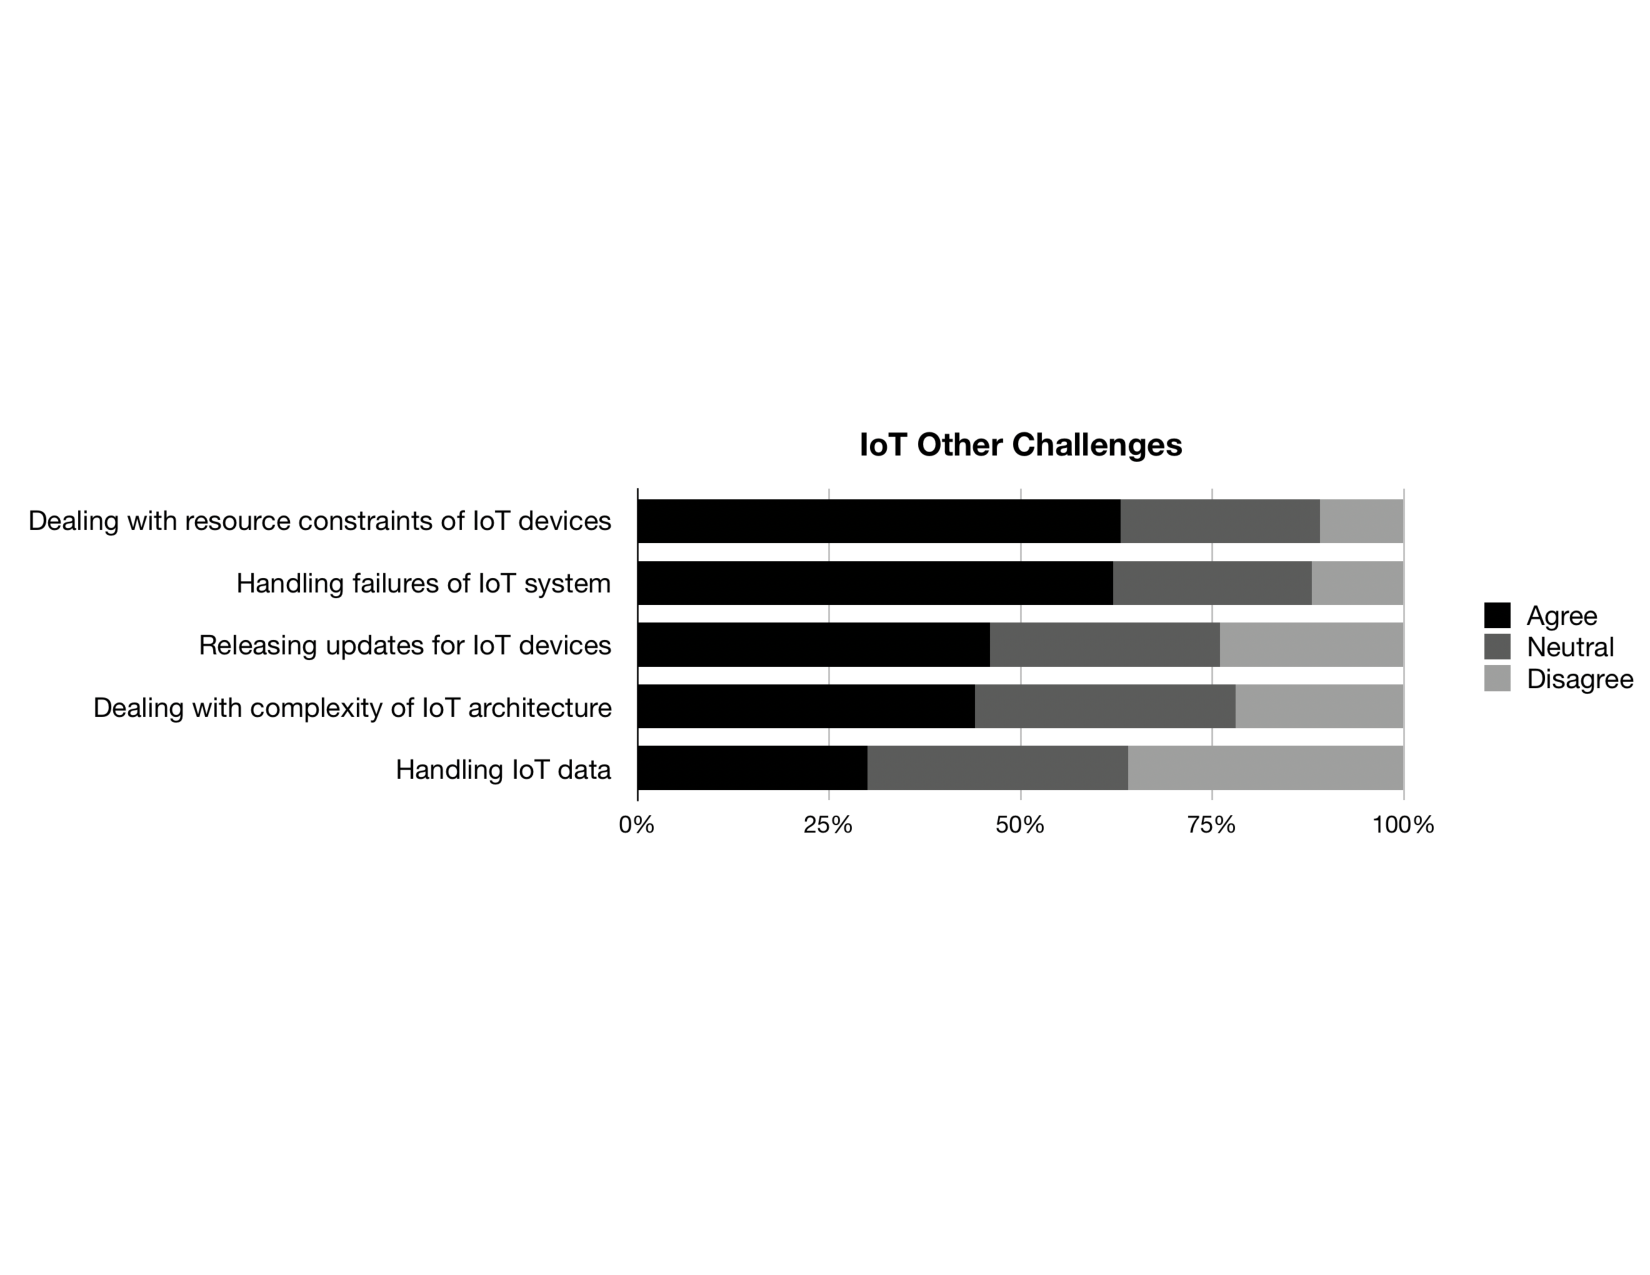
\includegraphics[width=\linewidth]{imgs/survey4}
  \caption{Survey responses about other IoT development challenges.}
  \label{fig:survey4}
\end{figure}

\section{Discussion}
\textbf{IoT testing solutions are not adopted in practice}
Various IoT testing tools and methods~\cite{testingtools2018}~\cite{pontes2018test} have been proposed in the literature, such as device simulators~\cite{iotify} and emulators~\cite{looga2012mammoth}, IoT unit testing frameworks~\cite{ArduinoUnit,platformio}, and IoT testbeds~\cite{iottestbed}. However, none of them seems to be adopted by IoT developers as only 9\% of them mentioned using third-party services as their main testing approach. Besides, although IoT test automation frameworks exist~\cite{iotify}, IoT testing is still carried out in a manual and ad-hoc manner, as 95\% of the IoT developers in our study perform manual testing practices. Also, as it is mentioned by P\textsubscript{5,8}, device simulation does not support simulating all types of devices. One possible future direction is having device simulators and emulators specifically crafted for each IoT device individually to virtualize their characteristics and bypass the need for the presence of the actual hardware device during testing. Also, as the importance of combinatorial testing in the context of IoT has been discussed previously in the literature~\cite{voas2018testing}, more focus is needed on combinatorial testing tools that consider the heterogeneous nature of IoT devices and protocols.

\textbf{Lack of device-level monitoring tool support}
Investigating the log data of IoT devices is a common debugging task for IoT developers. This task becomes even more important as the device status issues are among the most frequent bug categories. This bug category has appeared in around half of the bug reports in our dataset, and most IoT developers reported that they need to log communications or internal executions of the device as part of the debugging process for these bugs (P\textsubscript{1,2,3,4,7}). There is no universal tool that receives log data from all types of devices, and developers often have to manually employ naive approaches to monitor device status and communications, such as serial print for each device separately (P\textsubscript{2,7}) or using general-purpose tools like Wireshark (P\textsubscript{3,7}). Existing logging solutions to track devices are believed to be inefficient as their limitations were discussed by several IoT developers. One IoT developer best mentioned it as "\emph{even if some devices provide log libraries and tools, they should be manually aggregated or traced from each component separately to track an issue.}"

\textbf{Fragmented and ever-changing ecosystem of IoT}
One of the most serious challenges of IoT development nowadays is the rapid obsolescence of hardware devices. As several IoT experts and blog posts~\cite{gizmodoblogpost,iotforallblogpost} describe it, the pace that IoT devices get obscured and stop being supported by the providers is increasing. New updates for IoT devices often make the older devices unusable while they also break IoT developers' implementations. Within this ever-changing ecosystem of IoT, developers have to struggle with maintaining their device-specific or protocol-specific code. IoT developers, not only have to afford all versions of devices to keep up with these changes but also they have to allocate much of their development effort into migrating from one version or ecosystem to the other. As this issue targets both IoT consumers and developers, in 2019, some countries put regulations on the minimum time that IoT providers can release updates after the device is bought~\cite{UKregulations}. Furthermore, some solutions such as contract-based testing were suggested by interviewees (P\textsubscript{5}), to ensure continuous compatibility with third-party systems. However, none of these methods can be a long-term and universal solution as they are still dependent on the contracts and regulations in place.

\subsection{Threats to Validity}
\textbf{Internal validity}
One internal threat to the validity of our study, similar to most qualitative studies, is researchers' bias in coding qualitative data. We mitigated this risk by having all authors of the paper involved in the tagging process and discuss any discrepancies in tags for all pieces of qualitative data from various sources (bug reports, interview transcripts, survey comments). For interviews specifically, we eliminated any personal preference on our results by triangulation; each piece of meaningful data from interview transcripts was tagged by one researcher who conducted the interview and one who was not present in the interview session.

\textbf{External validity}
One external threat to the validity of our study is the generalization of studied IoT repositories. We minimized this issue by studying a large number of repositories (91 repositories) selected from all layers of IoT systems. Another risk to the validation of our study is the interview and survey participants not being representative of all IoT developers. However, we minimized this risk by recruiting interview and survey participants with different IoT-related field of expertise, years of experience, companies, and domains. In addition, our survey is filled out by 194 IoT developers with a diverse distribution of skills and experiences.

All our study material, including the bug dataset and interview and survey questions, is available online~\cite{repPack}.



\endinput

